\documentclass[noinstructornotes]{ximera}
%handout:  for handout version with no solutions or instructor notes
%handout,instructornotes:  for instructor version with just problems and notes, no solutions
%noinstructornotes:  shows only problem and solutions

%% handout
%% space
%% newpage
%% numbers
%% nooutcomes

%I added the commands here so that I would't have to keep looking them up
%\newcommand{\RR}{\mathbb R}
%\renewcommand{\d}{\,d}
%\newcommand{\dd}[2][]{\frac{d #1}{d #2}}
%\renewcommand{\l}{\ell}
%\newcommand{\ddx}{\frac{d}{dx}}
%\everymath{\displaystyle}
%\newcommand{\dfn}{\textbf}
%\newcommand{\eval}[1]{\bigg[ #1 \bigg]}

%\begin{image}
%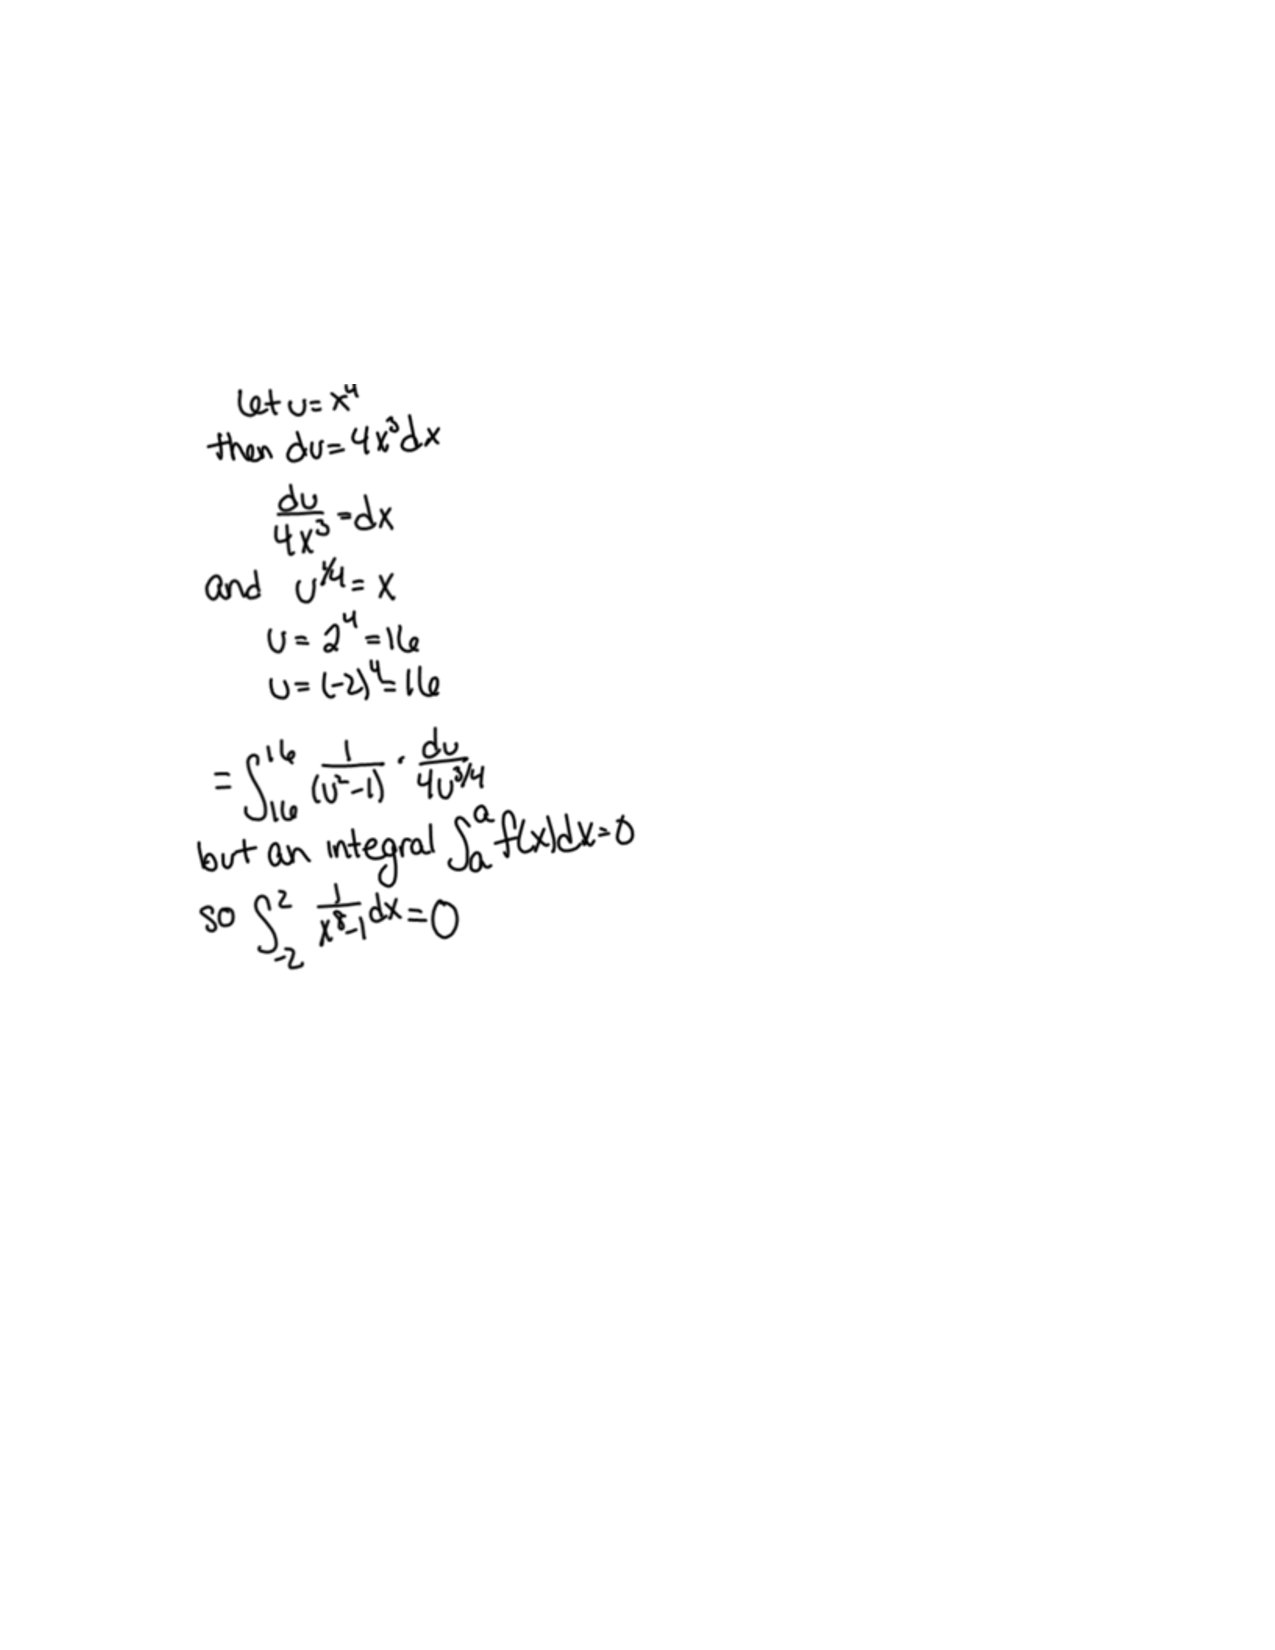
\includegraphics[trim= 170 420 250 180]{Figure1.pdf}
%\end{image}

%add a ``.'' below when used in a specific directory.
\newcommand{\RR}{\mathbb R}
\renewcommand{\d}{\,d}
\newcommand{\dd}[2][]{\frac{d #1}{d #2}}
\renewcommand{\l}{\ell}
\newcommand{\ddx}{\frac{d}{dx}}
\newcommand{\dfn}{\textbf}
\newcommand{\eval}[1]{\bigg[ #1 \bigg]}

\usepackage{multicol}

\renewenvironment{freeResponse}{
\ifhandout\setbox0\vbox\bgroup\else
\begin{trivlist}\item[\hskip \labelsep\bfseries Solution:\hspace{2ex}]
\fi}
{\ifhandout\egroup\else
\end{trivlist}
\fi} %% we can turn off input when making a master document

\title{Section 9.5: The Divergence, Integral, Ratio and Root Tests - Solutions}  

\begin{document}
\begin{abstract}		\end{abstract}
\maketitle












\section{Warm-Up}




%problem 1
\begin{problem}
	\begin{enumerate}
	
	\item  Why can we not use the Comparison test with $\sum_{k=1}^\infty \frac{1}{k^2}$ to show that $\sum_{k=1}^\infty \frac{1}{k^2 - 5}$ converges?
	
	\item  Adjust $\sum_{k=1}^\infty \frac{1}{k^2}$ to show that $\sum_{k=1}^\infty \frac{1}{k^2 - 5}$ converges via the Comparison Test.
	
	\item  Give a convergent series we can use in the Limit Comparison Test to show that $\sum_{k=1}^\infty \frac{1}{k^2 - 5}$ converges.  
	
	\end{enumerate}
	
	\begin{freeResponse}
		\begin{enumerate}
		
		\item  We cannot use the Comparison Test here because 
			\[
			\frac{1}{k^2} < \frac{1}{k^2 - 5}
			\]
		for all $k \geq 1$.  So we would just be showing the the series in question is greater than a series which converges, which does not give us any information.
		
		
		
		\item  Notice that
			\[
			\frac{2}{k^2} > \frac{1}{k^2 - 5}
			\]
		for all $k \geq 4$.  
		Since $\sum_{k=1}^\infty \frac{1}{k^2}$ converges, $\sum_{k=1}^\infty \frac{2}{k^2} = 2 \sum_{k=1}^\infty \frac{1}{k^2}$.  
		Thus, $\sum_{k=1}^\infty \frac{2}{k^2}$ converges.
		
		Therefore, the Comparison Test with $\sum_{k=1}^\infty \frac{2}{k^2}$ shows that $\sum_{k=0}^\infty \frac{1}{k^2-5}$ converges.
		
		
		
		\item  For the Limit Comparison Test, we \dfn{can} use $\sum_{k=1}^\infty \frac{1}{k^2}$.  
			\begin{align*}
			\lim_{k \to \infty} \frac{\frac{1}{k^2-5}}{\frac{1}{k^2}}
			&= \lim_{k \to \infty} \frac{k^2}{k^2-5}  \\
			&= 1.
			\end{align*}
			
		Thus, since $\sum_{k=1}^\infty \frac{1}{k^2}$ converges, by the Limit Comparison Test we know that $\sum_{k=0}^\infty \frac{1}{k^2-5}$ converges.
		
		\end{enumerate}
	\end{freeResponse}

\end{problem}

\begin{instructorNotes}
This problem may be done as a quick whole class discussion.  
For (b), use something like $\frac{2}{k^2}$.  
Be sure to determine for which $k$ the inequality will hold.
\end{instructorNotes}

%problem 2
\begin{problem}
For each of the following, answer {\bf True} or {\bf False}, and explain why.
	\begin{enumerate}
	
	\item  If $\sum_{n=0}^\infty a_n$ converges, then $\sum_{n=0}^\infty (a_n + 0.001)$ converges.
	
	\item  Since $\int_1^\infty x \sin(\pi x) \d x$ diverges then, by the Integral Test, $\sum_{n=0}^\infty n \sin(\pi n)$ diverges.
	
	\item  Since $\int_1^\infty \frac{1}{x^2} \d x = 1$ then, by the Integral Test, $\sum_{k=1}^\infty \frac{1}{k^2} = 1$.  
	
	\end{enumerate}
	
	\begin{freeResponse}
		\begin{enumerate}
		
		\item  {\bf False}
		
		Since $\sum_{n=0}^\infty a_n$ converges, we know that $\lim_{n \to \infty} a_n = 0$.  
		But then 
			\[
			\lim_{n \to \infty} (a_n + 0.0001) = 0.0001 \neq 0
			\]
		and so $\sum_{n=0}^\infty (a_n + 0.001)$ diverges by the Divergence Test.
		
		
		
		\item  {\bf False}
		
		The Integral Test only holds for positive, decreasing functions.  
		The function $f(x)= x \sin(\pi x)$ is not always positive, nor is it always decreasing.  
		So the Integral Test does not apply here.
		
		This problem is simpler than that though.  
		Since $\sin(\pi n) = 0$ for all integers $n$, we have that $\sum_{n=0}^\infty n \sin(\pi n) = 0$.
		
		
		
		\item  {\bf False}
		
		The Integral Test tells us that $\sum_{k=1}^\infty \frac{1}{k^2}$ converges, but it does {\bf not} give us the sum (this sum is actually $\frac{\pi^2}{6}$).  
		
		\end{enumerate}
	\end{freeResponse}
	
\end{problem}

\begin{instructorNotes}
For part (b) we need $f(x)$ to be a decreasing function for the Integral Test to (necessarily) hold.
All groups should do all of the parts.
\end{instructorNotes}





\section{Group work:}

%problem 3
\begin{problem}
Assume $\sum_{k=0}^\infty a_k =L$ and $b_k = 8$ for all $k$. 
	\begin{enumerate}
	
	\item  What is $\lim_{k \to \infty} (a_k + b_k)$?
	
	\item  What is $\lim_{k \to \infty} \sum_{n=0}^k (a_n + b_n)$?
	
	\item  What is $\lim_{k \to \infty} \sum_{n=0}^k (a_{n+1} - a_n)$?
	
	\end{enumerate}
	
	\begin{freeResponse}
		\begin{enumerate}
	
		\item  Since $\sum_{k=0}^\infty a_k$ converges, we know that $\lim_{k \to \infty} a_k = 0$.  
		Therefore,
			\[
			\lim_{k \to \infty} (a_k + b_k) = 0 + 8 = \boxed{8}.
			\]
	
		\item  Since $\lim_{n \to \infty} (a_n + b_n) = 8$, the series $\sum_{n=0}^\infty (a_n + b_n)$ diverges by the Divergence Test.  
		But $\lim_{k \to \infty}  \sum_{n=0}^k (a_n + b_n) = \sum_{n=0}^\infty (a_n + b_n)$.  
		Thus
			\[
			\lim_{k \to \infty}  \sum_{n=0}^k (a_n + b_n) = \sum_{n=0}^\infty (a_n + b_n) = \boxed{\infty}.
			\]
	
		\item  Let $S_k = \sum_{n=0}^k (a_{n+1} - a_n)$ (and recall that $\{ S_k \}$ is the {\it sequence of partial sums}).
		Then
			\begin{align*}
			S_k &= \sum_{n=0}^k (a_{n+1} - a_n)  \\
			&= (a_1 - a_0) + (a_2 - a_1) + (a_3 - a_2) + \hdots + (a_k - a_{k-1}) + (a_{k+1} - a_k)  \\
			&= a_{k+1} - a_0.
			\end{align*}
		Thus,
			\[
			\lim_{k \to \infty} \sum_{n=0}^k (a_{n+1} - a_n) = \lim_{k \to \infty} S_k = \lim_{k \to \infty} a_{k+1} - a_0 = \boxed{-a_0}.
			\]
	
		\end{enumerate}
	\end{freeResponse}
		
\end{problem}

\begin{instructorNotes}
This question was adapted from midterm \#2 in Spring 2013.  
Students had difficulty distinguishing between a question dealing with sequences vs. a question dealing with series.
\end{instructorNotes}





%Root and Ratio Test Problem
%problem 1
\begin{problem}
Determine if the following series converge or diverge.
	\begin{enumerate}
	
	\item  $\sum_{n=1}^\infty \frac{(7n+1)^2 \cdot 2^n}{5^n}$
	
	\item  $\sum_{n=1}^\infty a_n$, where $a_{n+1} = \frac{2n+5}{3n-1} \cdot a_n$ and $a_1 = 1$.
	
	\item  $\sum_{n=0}^\infty \frac{n^2 + 2n + 1}{3n^2 +1}$
	
	\item  $\sum_{n=2}^\infty \frac{1}{n(\ln n)^2}$
	
	\item $\sum_{k=1}^{\infty} \frac{(k!)^3}{(3k)!}$
	
	\end{enumerate}
	
	\begin{freeResponse}
		\begin{enumerate}
	
		\item  \dfn{Ratio Test}
			\begin{align*}
			\lim_{n \to \infty} \frac{a_{n+1}}{a_n} 
			&= \lim_{n \to \infty} \left[ \frac{(7(n+1) + 1)^2 \cdot 2^{n+1}}{5^{n+1}} \cdot \frac{5^n}{(7n+1)^2 \cdot 2^n} \right]  \\
			&= \lim_{n \to \infty} \frac{(7n+8)^2 \cdot 2}{5 \cdot (7n+1)^2}  \\
			&= \frac{49 \cdot 2}{49 \cdot 5} = \frac{2}{5}.
			\end{align*}
		Thus, since $\lim_{n \to \infty} \frac{a_{n+1}}{a_n} < 1$, this series \boxed{converges}.  
		
		
	
		\item  \dfn{Ratio Test}
		
		Even though the terms in this series look a little weird, this is set up perfectly for the Ratio Test:
			\[
			\lim_{n \to \infty} \frac{a_{n+1}}{a_n} = \lim_{n \to \infty} \frac{2n+5}{3n-1} = \frac{2}{3}.
			\]
		Thus, since $\lim_{n \to \infty} \frac{a_{n+1}}{a_n} < 1$, this series \boxed{converges}.  
		
		
	
		\item  \dfn{Divergence Test}
		
		Notice that
			\[
			\lim_{n \to \infty} a_n = \lim_{n \to \infty} \frac{n^2 + 2n + 1}{3n^2 +1} = \frac{1}{3}.
			\]
		Therefore, since $\lim_{n \to \infty} a_n \neq 0$, by the Divergence Test this series \boxed{diverges}.
		
		
	
		\item  \dfn{Integral Test}
		
		First, notice that $f(x) = \frac{1}{x (\ln x)^2}$ is a decreasing and positive function on $[2,\infty)$.
		Then
			\begin{align*}
			\int_2^\infty f(x) \d x 
			&= \int_2^\infty \frac{1}{x (\ln x)^2} \d x  \\
			&= \lim_{b \to \infty} \int_2^b \frac{1}{x (\ln x)^2} \d x  \\
			&= \lim_{b \to \infty} \int_{\ln 2}^{\ln b} u^{-2} \d u  \quad  {\color{red} u = \ln x, \d u = \frac{1}{x} \d x}  \\
			&= \lim_{b \to \infty} \eval{\frac{-1}{u}}_{\ln 2}^{\ln b}  \\
			&= \lim_{b \to \infty} \left( \frac{-1}{\ln b} + \frac{1}{\ln 2} \right)  \\
			&= 0 + \frac{1}{\ln 2} = \frac{1}{\ln 2}.
			\end{align*}
		Therefore, since the above integral converges, the series $\sum_{n=2}^\infty \frac{1}{n(\ln n)^2}$ \boxed{converges} by the Integral Test.
	

		\item \dfn{Ratio Test}
		\begin{align*}
			\lim_{k \to \infty} \frac{a_{k+1}}{a_k} 
			&= \lim_{k \to \infty} \left[ \frac{( (k+1)!)^3}{(3(k+1))!}  \cdot \frac{(3k)!}{(k!)^3} \right]  \\
			&= \lim_{k \to \infty} \frac{ (k+1)^3 (k!)^3}{(3k+3)(3k+2)(3k+1) \cdot (3k)!} \cdot \frac{(3k)!}{(k!)^3} \\
			&= \lim_{k \to \infty} \frac{(k+1)^3}{(3k+3)(3k+2)(3k+1)}  \\
			&= \frac{1}{3 \cdot 3 \cdot 3}= \frac{1}{27}.
			\end{align*}
		Thus, since $\lim_{k \to \infty} \frac{a_{k+1}}{a_k} < 1$, this series \boxed{converges}. 
		
		\end{enumerate}
	\end{freeResponse}
	
\end{problem}

\begin{instructorNotes}
Let the students experiment with what tests to use.  
Perhaps give two problems per group.
\end{instructorNotes}







\begin{problem}
Determine if the following series converge or diverge.
	\begin{multicols}{2}
	\begin{enumerate}
	
	\item  $\sum_{n=0}^\infty \frac{n^2 + 2n + 1}{3n^3+1}$
	
	\item  $\sum_{n=0}^\infty \frac{n^2+2n+1}{3n^4+1}$
	
	\item  $\sum_{n=0}^\infty \frac{\cos^2 n}{n^3+1}$
	
	\item  $\sum_{n=1}^\infty \left[ \left( 1+\frac{1}{n} \right)^2 e^{-n} \right]$
	
	\end{enumerate}
	\end{multicols}
	
	\begin{freeResponse}
		\begin{enumerate}
		
		\item  Use the \dfn{Limit Comparison Test} with $\sum_{n=1}^\infty \frac{1}{n}$.
			\begin{align*}
			\lim_{n \to \infty} \frac{a_n}{b_n}
			&= \lim_{n \to \infty} \frac{n^2+2n+1}{3n^3+1} \cdot \frac{n}{1}  \\
			&= \frac{1}{3}.
			\end{align*}
			
		Therefore, since $\sum_{n=1}^\infty \frac{1}{n}$ diverges, by the Limit Comparison Test we know that $\sum_{n=0}^\infty \frac{n^2+2n+1}{3n^3+1}$ diverges.
		
		
		
		\item  Use the \dfn{Limit Comparison Test} with $\sum_{n=1}^\infty \frac{1}{n^2}$.
			\begin{align*}
			\lim_{n \to \infty} \frac{a_n}{b_n}
			&= \lim_{n \to \infty} \frac{n^2+2n+1}{3n^4+1} \cdot \frac{n^2}{1}  \\
			&= \frac{1}{3}.
			\end{align*}
			
		Therefore, since $\sum_{n=1}^\infty \frac{1}{n^2}$ converges, by the Limit Comparison Test we know that $\sum_{n=0}^\infty \frac{n^2+2n+1}{3n^4+1}$ converges.
		
		
		
		\item  Use the \dfn{Comparison Test} with $\sum_{n=1}^\infty \frac{1}{n^3}$.  
		
		Since we always have that $0 < \cos^2(n) < 1$, we know that
			\[
			\frac{\cos^2(n)}{n^3 + 1} \leq \frac{1}{n^3+1} < \frac{1}{n^3}.
			\]
		Therefore, by the Comparison Test, we have that $\sum_{n=0}^\infty \frac{\cos^2 n}{n^3+1}$ converges.
		
		
		
		\item  Use the \dfn{Comparison Test} with $\sum_{n=1}^\infty 2 \cdot e^{-n}$.
		
		First, notice that for all $n \geq 3$,
			\[
			\left( 1 + \frac{1}{n} \right)^2 < 2.
			\]		
		Also, notice that $\sum_{n=1}^\infty e^{-n}$ is a convergent geometric series.  
		Therefore $\sum_{n=1}^\infty 2 \cdot e^{-n}$ converges, and so $\sum_{n=1}^\infty \left[ \left( 1+\frac{1}{n} \right)^2 e^{-n} \right]$ converges by the Comparison Test.
		
		\end{enumerate}
	\end{freeResponse}

\end{problem}

\begin{instructorNotes}
These are all done using either the Comparison Test or the Limit Comparison Test.  
Parts (a) and (b) should be done with the limit comparison test (explain why).  
It is important to compare and contrast these two problems.  
Parts (c) and (d) should be done with the Comparison Test (again, explain why).  
The $e^{-n}$ should be treated as a geometric series.
\end{instructorNotes}
















	
	
	
	
	
	
	
	
	

	










								
				
				
	














\end{document} 


















